%\documentclass{beamer}
%\usepacakge[UTF8]{ctex}
%----------------------------------------------------------------------------------------
%    PACKAGES AND THEMES
%----------------------------------------------------------------------------------------

\documentclass[aspectratio=169,xcolor=dvipsnames]{beamer}
\usepackage[UTF8]{ctex}
\usetheme{SimplePlus}
\setbeamertemplate{footline}{}

\usepackage{hyperref}
\usepackage{graphicx} % Allows including images
\graphicspath{{./images/}}
\usepackage{booktabs} % Allows the use of \toprule, \midrule and \bottomrule in tables

\usepackage{mathpartir}

\usepackage{tikz}
\usetikzlibrary{calc}

\usepackage{tabularx}

\usepackage{tikz-cd}
\usetikzlibrary{arrows.meta}
%\tikzcdset{arrow style=tikz, diagrams={>=Stealth}}

\usepackage{fontspec}

\newcommand\calV{\mathcal{V}}
\newcommand\calU{\mathcal{U}}
\newcommand\bfC{\mathbf{C}}
\newcommand\calE{\mathcal{E}}
\newcommand\bbD{\mathbb{D}}
\newcommand\bbI{\mathbb{I}}
\newcommand\bbF{\mathbb{F}}
\newcommand\JEq{\mathtt{JEq}}
\newcommand\FTy{\mathtt{FTy}}
\newcommand\Fill{\mathtt{Fill}}
\newcommand\ttfill{\mathtt{fill}}
\newcommand\isFib{\mathtt{isFib}}
\newcommand\comp{\mathtt{comp}}
\newcommand\Comp{\mathtt{Comp}}
\newcommand\fst{\mathtt{fst}}
\newcommand\snd{\mathtt{snd}}
\newcommand\Ty{\mathtt{Ty}}
\newcommand\ttI{\mathtt{I}}
\newcommand\Ter{\mathtt{Ter}}
\newcommand\Path{\mathtt{Path}}
\newcommand\dM{\mathsf{dM}}
\newcommand\ttp{\mathtt{p}}
\newcommand\ttq{\mathtt{q}}
\newcommand\bfone{\mathbf{1}}
\newcommand\ttzero{\mathtt{0}}
\newcommand\ttone{\mathtt{1}}
\newcommand\Set{\mathbf{Set}}
\newcommand\DM{\mathbf{DM}}
\newcommand\Id{\mathtt{Id}}
\newcommand\refl{\mathtt{refl}}
\newcommand\C{\mathbf{C}}
\newcommand\psC{\widehat{\mathbf{C}}}
\newcommand\extop{{\scalebox{0.4}[1]{\_}}.{\scalebox{0.8}[1]{\_}}}
\newcommand{\shortminus}{\raisebox{0.3ex}{\scalebox{0.8}[1.0]{-}}}
\newcommand{\mathshortminus}{\mathbin{\text{\normalfont\shortminus}}}
\newcommand{\ul}{{\scalebox{0.4}[0.4]{\_}}}
\newcommand{\ax}[1]{\mathbf{ax_{#1}}}
\newcommand\uc{\mathtt{uc}}

\DeclareMathOperator\FreeDeMorgan{FreeDeMorgan}
\DeclareMathOperator\obj{obj}
\DeclareMathOperator\y{\mathbf{y}}
%\newcommand\cof{\mathtt{cof}}
\newcommand\Cof{\mathtt{Cof}}
\DeclareMathOperator\cof{\mathtt{cof}}
\DeclareMathOperator\cofibpart{\square}
\DeclareMathOperator\Fib{\mathtt{Fib}}

\usepackage{unicode-math}
%\setmathfont{Latin Modern Math}
%\setmathfont{XITS Math}[range=cal]
%\setmathfont{Euler Math}[range=cal]

\DeclareMathAlphabet{\mathcal}{OMS}{cmsy}{m}{n}

\newcommand\cubicalsets{\widehat{□}}

\usepackage{mathpartir}

\usepackage{framed}

\newfontfamily{\codefont}{Unifont}
% 设置 verbatim 默认字体
\makeatletter
\renewcommand{\verbatim@font}{\codefont\small}  % 替换为实际的Unifont命令
\makeatother

%----------------------------------------------------------------------------------------
%    TITLE PAGE
%----------------------------------------------------------------------------------------

\title{使用 Agda 形式化}
%\subtitle{Subtitle}

%\author{Pin-Yen Huang}

%\institute
%{
%    Department of Computer Science and Information Engineering \\
%    National Taiwan University % Your institution for the title page
%}
%\date{\today} % Date, can be changed to a custom date
\date{}

%----------------------------------------------------------------------------------------
%    PRESENTATION SLIDES
%----------------------------------------------------------------------------------------

\begin{document}

\begin{frame}
    % Print the title page as the first slide
    \titlepage
\end{frame}

\begin{frame}{背景}
  在拓扑斯的内部类型理论中工作, 而不是从外部处理拓扑斯的对象和态射, 这种方法的一个优点是它更适合机器辅助形式化. 要理解为什么, 可以考虑形式化一个从外部构建的模型会涉及什么. 首先, 我们需要定义所有的数学结构(范畴、函子等)并形式化模型构建中使用的所有相关属性. 接下来, 我们必须形式化模型本身, 使用前一步中定义的结构. 通过在内部语言中工作, 我们基本上可以去掉整个第一步. 这是因为, 我们不是在证明助手中形式化拓扑斯的概念及其内部语言, 而是简单地将证明助手当作拓扑斯的内部语言来使用.
\end{frame}

\begin{frame}[fragile,shrink]{拓扑斯内部语言和 Agda 的区别}
  \begin{itemize}
  \item Agda 的相等类型是内涵性的, 而内部类型理论的相等类型是外延性的. 这意味着我们在形式化过程中需要做更多的工作. 例如, 我们可能需要在命题相等的类型之间进行显式强制转换, 而这在内部语言中是隐式的.
  \item Agda 默认情况下不包含一个与子对象分类子 $Ω$ 对应的非直谓性命题全集.
  \begin{verbatim}

   {-# OPTIONS --type-in-type #-}
   record Ω : Set where
     constructor prop
     field
       prf : Set
       equ : (u v : prf) → u ≡ v
  \end{verbatim}
  我们仅将 \verb|type-in-type| 用于 $Ω$ 的定义, 并且该定义被分离到一个单独的模块中, 而 \verb|type-in-type| 选项在该模块之外不被启用, 我们相信这种受限的使用是相容的.
\end{itemize}
\end{frame}

\begin{frame}[fragile,shrink]{余纤维化}
  考虑一类单态射 $m : A\rightarrowtail B$, 其分类态射
  \[
  \chi_m \triangleq \lambda(y:B)\to\exists(x:A). m\,x = y : B \to \Omega
  \]
  可以通过 $\Cof\rightarrowtail\Omega$ 进行分解. 我们称此类单态射为余纤维化.
  \[
  \forall b:B, \cof(\chi_m(b))
  \]
  \[
  \begin{tikzcd}[row sep = tiny]
  A \arrow[r,tail, "m"] \arrow[dd] & B \arrow[dd,"{\chi_m}"] \arrow[dr] & \\
  & & \Cof \arrow[dl,tail] \\
  1 \arrow[r,"\top"] & \Omega &
  \end{tikzcd}
  \]
\end{frame}

\begin{frame}[shrink]{$\ax{7}:[\forall(\varphi\:\psi:\Omega).\cof\varphi\Rightarrow(\varphi\Rightarrow\cof\psi)\Rightarrow\cof(\varphi\land\psi)]$}
  公理 $\ax{7}$ 等价于要求余纤维化在组合运算下封闭.

  %\bigskip
  首先假设$\ax{7}$成立, 并且$f:A\rightarrowtail B$和$g:B\rightarrowtail C$ 是余纤维化. 因此(根据余纤维化的定义, 其分类态射可以通过 $\Cof\rightarrowtail\Omega$ 进行分解)
  \begin{itemize}
    \item $\forall(b:B).\cof(\exists(a:A).f\,a=b)$
    \item $\forall(c:C).\cof(\exists(b:B).g\,b=c)$
  \end{itemize}
  都成立, 并且我们希望证明$\forall(c:C).\cof(\exists(a:A).g(f\,a)=c)$. 注意到, 对于 $b:B$ 和 $c:C$
  \begin{align*}
    g\,b=c \quad&\stackrel{g\text{是单态射}}{\implies}\quad (\exists(a:A).g(f\,a)=c) = (\exists(a:A).f\,a=b) \\
    &\stackrel{\phantom{g\text{是单态射}}}{\implies}\quad \cof(\exists(a:A).g(f\,a)=c) = \cof(\exists(a:A).f\,a=b) = \top
  \end{align*}
  因此对于$\varphi\triangleq\exists(b:B).g\,b=c$和$\psi\triangleq\exists(a:A).g(f\,a)=c$, 我们有$\cof\varphi$且$\varphi\Rightarrow\cof\psi$. 因此根据 $\ax{7}$, 我们得到$\cof(\varphi\land\psi)$, 它等于 $\cof\psi$ 因为 $\psi\Rightarrow\varphi$. 所以我们确实有 $\forall(c:C).\cof(\exists(a:A).g(f\,a)=c)$.
\end{frame}

\begin{frame}{唯一选择公理}
  \[
  \uc : (\varphi : A \to \Omega) \to [\exists!(a:A).\varphi\,a]\to\{a:A\mid\varphi\,a\}
  \]
  其中$\exists!(a:A).\varphi\,a\triangleq\exists(a:A).(\varphi\,a\land\forall(a':A).\varphi\,a'\Rightarrow a=a')$.
\end{frame}

\begin{frame}[fragile,shrink]{余纤维部分元素 $\cofibpart A$}
  我们称类型 $\Cof$ 的元素为\emph{余纤维命题}. 给定一个类型 $A:\calU$, 我们将$A$的余纤维部分元素的类型定义为:
  \[
  \cofibpart A \triangleq (\varphi : \Cof) \times ([\varphi]\to A)
  \]
  这样一个部分元素 $(\varphi,f):\cofibpart A$ 的一个扩张是一个元素 $a:A$ 并满足如下定义
  \[
  (\varphi,f) \nearrow a \triangleq \forall(u:[\varphi]).f\,u=a
  \]
\end{frame}

\begin{frame}[fragile,shrink]{例}
  将类型$\ttI$的变量看作空间中的维度名称是有帮助的, 因此在一个上下文 $i_1,\ldots,i_n : \ttI$ 中工作对应于在 $n$ 维空间中工作. 假设我们正在一个包含 $i,j,k : \ttI$ 的上下文中工作, 那么这就对应于在三维空间中工作. 我们将一个元素 $i,j,k:\ttI\vdash a:A$ 看作是空间 $A$ 中的一个立方体

  \begin{tikzpicture}[scale=0.3]
   \draw[->] (0,0,0) -- (3,0,0) node[right] {$j$};
   \draw[->] (0,0,0) -- (0,3,0) node[above] {$i$};
   \draw[->] (0,0,0) -- (0,0,-4.2) node[right] {$k$};
   %\draw[thick,black]  (4,0,0) -- (4,0,-4) -- (4,4,-4) -- (4,4,0) -- cycle;
   %\draw[thick,black](0,4,0) -- (0,4,-4) -- (4,4,-4);
   \node at (1.5,-2,0) {$i,j,k:\mathtt{I}$};

  \end{tikzpicture}
  \qquad
  \begin{tikzpicture}[scale=0.3]

   \draw[style=dashed, color=black] (4,0,-4) -- (0,0,-4)-- (0,4,-4);
   \draw[style=dashed, color=black] (0,0,0) -- (0,0,-4); 
   %\draw[<->](0,-0.3,0)--(4,-0.3,0);
   %\draw node[below] at (2,-0.3,0) {c}; 

   \fill[gray!50,opacity=0.6](4,0,0) -- (0,0,0) -- (0,4,0) -- (4,4,0);
   \fill[gray!50,opacity=0.6](4,0,0) -- (4,0,-4) -- (4,4,-4) -- (4,4,0);
   \fill[gray!50,opacity=0.6](0,4,0) -- (0,4,-4) -- (4,4,-4) -- (4,4,0);

   \draw[black] (4,0,0) -- (0,0,0) -- (0,4,0) -- (4,4,0);
   \draw[black]  (4,0,0) -- (4,0,-4) -- (4,4,-4) -- (4,4,0) -- cycle;
   \draw[black](0,4,0) -- (0,4,-4) -- (4,4,-4);

   \node at (2.2,-2,0) {$a:A$};
  \end{tikzpicture}

  令 $\varphi\triangleq(i=\ttzero)\lor(j=\ttzero)\lor(j=\ttone\land k=\ttone)$, 那么 $i,j,k:\ttI\vdash\varphi : \Cof$. 我们将 $\varphi$ 看作指定了立方体的某些面和边, 在本例中是底面$(i=\ttzero)$, 左面$(j=\ttzero)$以及右前棱$(j=\ttone\land k=\ttone)$. 那么, 一个余纤维部分元素 $f : [\varphi] \to A$ 可以被看作是一个部分立方体, 仅在由 $\varphi$ 指定的区域上有定义.

\begin{tikzpicture}[scale=0.3]
\coordinate (A) at (0,4,-4);
\coordinate (B) at (4,4,-4);
\coordinate (C) at (4,4,0);
\coordinate (D) at (0,4,0);
\coordinate (E) at (0,0,-4);
\coordinate (F) at (4,0,-4);
\coordinate (G) at (4,0,0);
\coordinate (H) at (0,0,0);
  \draw[black] (E) -- (F) -- (G) -- (H);
  \draw[black] (H) -- (D) -- (A) -- (E);
  \draw[black] (B) -- (F);

   %\draw[style=dashed, color=black] (0,0,0) -- (0,0,-4); 
   %\draw[<->](0,-0.3,0)--(4,-0.3,0);
   %\draw node[below] at (2,-0.3,0) {c}; 


   %\fill[blue!40!white,opacity=0.6](0,0,0) -- (4,0,0) -- (4,0,-4) -- (0,0,-4);
   \fill[gray!50,opacity=0.6](0,0,0) -- (4,0,0) -- (4,0,-4) -- (0,0,-4);
   \fill[gray!50,opacity=0.6](0,0,0) -- (0,4,0) -- (0,4,-4) -- (0,0,-4);
   %\draw[style=dashed, color=black] (A) -- (B) -- (C) -- (D);
   %\draw[style=dashed, color=black] (C) -- (G);

   \draw[->] (0,0,0) -- (5,0,0) node[right] {$j$};
   \draw[->] (0,0,0) -- (0,5,0) node[above] {$i$};
   \draw[->] (0,0,0) -- (0,0,-6.2) node[right] {$k$};
   \node at (2.2,-2,0) {$f:[\varphi]\to A$};
   \end{tikzpicture}
\end{frame}

\begin{frame}{同构}
  给定对象$A,B:\calU$, $A$和$B$之间的一个同构是一个函数$f:A\to B$, 它有一个双边逆. 令$A\cong B$为$A$和$B$之间的同构类型, 定义为
  \[
  A\cong B\triangleq \{f:A\to B\mid(\exists g:B\to A)(g\circ f=id)\land(f\circ g=id)\}
  \]
  如果存在一个同构$f:A\cong B$, 我们就说$A$和$B$是同构的. 如果两个类型族$A,B:\Gamma\to\calU$的每一个纤维都是同构的, 我们就说它们是同构的, 并且我们不太正规地写成
  \[
  A\cong B \triangleq (x:\Gamma)\to A\,x\cong B\,x
  \]
  同构的逆是相对于内部类型理论的外延等价而言的, 这与我们稍后将介绍的等价概念形成对比, 后者只具有相对于路径等价的逆. 此外, 这些逆是唯一的, 因此, 使用唯一选择, 我们总是可以构造一个同构的逆. 因此, 给定 $f : A ≅ B$, 我们将 $f⁻¹ : B ≅ A$ 写成 $f$ 的这个逆.
\end{frame}

\begin{frame}[shrink]{严格性公理}
  这条公理关注解决内部语言方法的弱点.

  \bigskip

  任何余纤维-部分类型 $A$, 如果在 $A$ 定义的任何地方都与全类型 $B$ 同构, 则可以扩展为与 $B$ 同构的全类型 $B'$:
  \begin{align*}
    \ax{9} :\ &\{\varphi:\Cof\}(A:[\varphi]\to\calU)(B:\calU)(s:(u:[\varphi])\to(A\,u\cong B)) \to \\
    &(B':\calU)\times\{s':B'\cong B\mid\forall(u:[\varphi]).\ A\,u=B'\land s\,u=s'\}
  \end{align*}
\end{frame}

\begin{frame}[fragile]{$\mathtt{I}$}
\begin{verbatim}
postulate
  Int   : Set
  O     : Int
  I     : Int
  O≠I   : O ≡ I → ∅
  min   : Int → Int → Int
  max   : Int → Int → Int
  cntd  : (P : Int → Ω) → ((i : Int) → prf(P i or ¬(P i))) → P O ≡ P I
\end{verbatim}
\end{frame}

\begin{frame}[fragile]{$\cof:\Omega\to\Omega$}
  \begin{verbatim}
postulate
  cof   : Ω → Ω
  cofO  : (i : Int) → prf (cof (i ≈ O))
  cofI  : (i : Int) → prf (cof (i ≈ I))
  cofor : (P Q : Ω) → prf (cof P ⊃ cof Q ⊃ cof(P or Q))
  cof&  : (P Q : Ω) → prf (cof P ⊃ (P ⊃ cof Q) ⊃ cof(P & Q))
  cof∀  : (P : Int → Ω) → prf ((All i ∈ Int , cof (P i)) ⊃ cof (All i ∈ Int , P i))

Cof : Set
Cof = ⟦ P ∈ Ω ∣ cof P ⟧

[_] : Cof → Set
[ φ ] = prf (fst φ)

  \end{verbatim}
\end{frame}

\begin{frame}[fragile,shrink]{}
\begin{verbatim}
----------------------------------------------------------------------
-- Cofibrant-partial function classifier
----------------------------------------------------------------------
□ : Set → Set
□ A = Σ φ ∈ Cof , ([ φ ] → A)

_↗_ : {A : Set} → □ A → A → Ω
(φ , f) ↗ x = All u ∈ [ φ ] , f u ≈ x

----------------------------------------------------------------------
-- Dependently typed paths
----------------------------------------------------------------------
Π : (Int → Set) → Set
Π A = (i : Int) → A i

Π′ :
  {A B : Int → Set}
  → ---------------------------------
  ((i : Int) → A i → B i) → Π A → Π B
Π′ F p i = F i (p i)

_∙_ :
  {A : Int → Set}
  → -------------------------
  □(Π A) → (i : Int) → □(A i)
(φ , f) ∙ i = (φ , λ u → f u i)

----------------------------------------------------------------------
-- Restricting a context by a cofibrant propositions
----------------------------------------------------------------------
res : ∀{a}(Γ : Set a)(Φ : Γ → Cof) → Set a
res Γ Φ = Σ x ∈ Γ , [ Φ x ]

\end{verbatim}
\end{frame}

\begin{frame}[fragile,shrink]{组合与填充结构}
  给定一个区间索引的类型族 $A : \ttI\to\calU$, 我们把依赖函数类型 $\Pi_{\ttI}A\triangleq(i:\ttI)\to A\,i$ 的元素看作是依赖类型的路径. 我们将类型$\cofibpart(\Pi_{\ttI}A)$的元素称为\emph{余纤维-部分路径}. 给定$(\varphi,f) : \cofibpart(\Pi_{\ttI}A)$, 我们可以在区间的某个点$i:\ttI$处对其求值, 以得到一个余纤维部分元素$(\varphi,f)\,@\,i : \cofibpart(A\,i)$:
  \[
  (\varphi,f)\,@\,i \triangleq (\varphi,\lambda(u:[\varphi])\to f\,u\,i)
  \]
  在$A : \ttI\to\calU$中一个\emph{从$\mathtt{0}$填充}的操作, 会取任意$(\varphi,f):\cofibpart(\Pi_{\ttI}A)$和任意$a_{\mathtt{0}}:A\,\mathtt{0}$ (其中$(\varphi,f)\,@\,\mathtt{0} \nearrow a_{\mathtt{0}}$), 并将 $(\varphi,f)$ 扩展为一个依赖类型的路径 $g:\Pi_{\ttI}A$, 且满足$g\,\mathtt{0} = a_{\mathtt{0}}$.

  由于我们没有假设区间上存在用于反转路径的任何结构, 我们还需要考虑从 $\ttone$ 填充的对称概念. 令
  \[
  \{\ttzero,\ttone\}\triangleq\{i:\ttI\mid i=0\lor i=1\}
  \]
  存在一个函数
  \[
  \overline{\phantom{\ttzero}} : \{ \ttzero, \ttone \} \to \{ \ttzero, \ttone \}
  \]
  满足 $\overline{\ttzero} = \ttone$ 和 $\overline{\ttone} = \ttzero$.

  在下文中, 我们将不使用路径反转, 而是用 $e:\{\ttzero,\ttone\}$ 来参数化定义, 并使用$\overline{\phantom{\ttzero}}$ 来交换$\ttzero$和$\ttone$.
\end{frame}

\begin{frame}[fragile,shrink]{填充结构}
  给定 $e : \{\ttzero,\ttone\}$, 一个$\ttI$-索引的类型族$A:\ttI\to\calU$的填充结构的类型 $\Fill\,e\,A : \calU$ 定义为:
  \begin{align*}
    \Fill\,e\,A\triangleq &(\varphi:\Cof)(f:[\varphi]\to\Pi_{\ttI}A)(a:\{a':A\,e\mid(\varphi,f)\,@\,e\nearrow a'\})\to \\
    &\{g:\Pi_{\ttI}A\mid(\varphi,f)\nearrow g\land g\,e=a\}
  \end{align*}
  为了直观理解为什么这样的操作被称为填充, 我们考虑下面的例子. 为简单起见, 假设 $A : \ttI \to \calU$ 是一个常量族 $A\triangleq\lambda(\ul:\ttI)\to A'$. 我们将类型 $\ttI$ 的变量看作空间中的维度, 因此, 给定一个在环境上下文 $j,k:\ttI$ 中的元素 $a:A$, 我们将其看作空间 $A$ 中的一个正方形. 我们感兴趣的是将这个二维正方形扩展为一个三维立方体. 让我们假设我们已经知道如何在立方体的某些面和边上扩展 $a$, 例如, 在由 $\varphi \triangleq (j=0) \lor (j=1\land k=1)$ 指定的面/边上. 这意味着我们有一个余纤维部分路径 $f:[\varphi]\to\Pi_{\ttI}A$, 它在它们共同定义的地方与$a$一致, 即$(\varphi,f)\,@\,\ttzero\nearrow a$. 这个数据的一个填充是一个立方体 $g : \Pi_{\ttI}A$, 它与我们开始的面/边一致. 也就是说, 它扩展了 $f$ 并且在立方体的底部与 $a$ 一致: $(\varphi,f)\nearrow g$ 并且 $g\,\ttzero = a$.
\end{frame}

\begin{frame}[fragile,shrink]{}
    \begin{tikzpicture}[scale=0.3]
   \draw[->] (0,0,0) -- (3,0,0) node[right] {$j$};
   \draw[->] (0,0,0) -- (0,3,0) node[above] {$i$};
   \draw[->] (0,0,0) -- (0,0,-4.2) node[right] {$k$};
   %\draw[thick,black]  (4,0,0) -- (4,0,-4) -- (4,4,-4) -- (4,4,0) -- cycle;
   %\draw[thick,black](0,4,0) -- (0,4,-4) -- (4,4,-4);
   \node at (1.5,-2,0) {$i,j,k:\mathtt{I}$};
  \end{tikzpicture}
  \qquad
\begin{tikzpicture}[scale=0.3]
\coordinate (A) at (0,4,-4);
\coordinate (B) at (4,4,-4);
\coordinate (C) at (4,4,0);
\coordinate (D) at (0,4,0);
\coordinate (E) at (0,0,-4);
\coordinate (F) at (4,0,-4);
\coordinate (G) at (4,0,0);
\coordinate (H) at (0,0,0);
  %\draw[thick,black] (E) -- (F) -- (G) -- (H) -- cycle;
  %\draw[thick,black] (A) -- (D) -- (H) -- (E) -- cycle;
  %\draw[thick,black] (B) -- (F);
  \draw[style=dashed, color=black] (A) -- (B) -- (C) -- (D) -- cycle;
  \draw[color=black] (E) -- (F) -- (G) -- (H) -- cycle;
   \draw[style=dashed, color=black] (C) -- (G);
   \draw[style=dashed, color=black] (A) -- (E);
   \draw[style=dashed, color=black] (B) -- (F);
   \draw[style=dashed, color=black] (D) -- (H);
   %\draw[style=dashed, color=black] (0,0,0) -- (0,0,-4); 
   %\draw[<->](0,-0.3,0)--(4,-0.3,0);
   %\draw node[below] at (2,-0.3,0) {c}; 


   %\fill[blue!40!white,opacity=0.6](0,0,0) -- (4,0,0) -- (4,0,-4) -- (0,0,-4);
   \fill[gray!50,opacity=0.6](E) -- (F) -- (G) -- (H);
   %\fill[gray!50,opacity=0.6](0,0,0) -- (0,4,0) -- (0,4,-4) -- (0,0,-4);

   \node at (2.2,-2,0) {$a : A$};
   \end{tikzpicture}
   \qquad
   \begin{tikzpicture}[scale=0.3]
\coordinate (A) at (0,4,-4);
\coordinate (B) at (4,4,-4);
\coordinate (C) at (4,4,0);
\coordinate (D) at (0,4,0);
\coordinate (E) at (0,0,-4);
\coordinate (F) at (4,0,-4);
\coordinate (G) at (4,0,0);
\coordinate (H) at (0,0,0);

  \draw[style=dashed, color=black] (A) -- (B) -- (C) -- (D);
  \draw[style=dashed, color=black] (E) -- (F) -- (G) -- (H);

   \draw[style=dashed, color=black] (C) -- (G);
   \draw[color=black] (A) -- (E);
   \draw[color=black] (B) -- (F);
   \draw[color=black] (D) -- (H);
   \draw[color=black] (D) -- (A);
   \draw[color=black] (H) -- (E);

   \fill[gray!50,opacity=0.6](A) -- (E) -- (H) -- (D);

   \node at (2.2,-2,0) {$f:[\varphi]\to\Pi_{\ttI}A$};
   \end{tikzpicture}
   \qquad
  \begin{tikzpicture}[scale=0.3]

   \draw[style=dashed, color=black] (4,0,-4) -- (0,0,-4)-- (0,4,-4);
   \draw[style=dashed, color=black] (0,0,0) -- (0,0,-4); 
   %\draw[<->](0,-0.3,0)--(4,-0.3,0);
   %\draw node[below] at (2,-0.3,0) {c}; 

   \fill[gray!50,opacity=0.6](4,0,0) -- (0,0,0) -- (0,4,0) -- (4,4,0);
   \fill[gray!50,opacity=0.6](4,0,0) -- (4,0,-4) -- (4,4,-4) -- (4,4,0);
   \fill[gray!50,opacity=0.6](0,4,0) -- (0,4,-4) -- (4,4,-4) -- (4,4,0);

  \draw[black] (4,0,0) -- (0,0,0) -- (0,4,0) -- (4,4,0);
   \draw[black]  (4,0,0) -- (4,0,-4) -- (4,4,-4) -- (4,4,0) -- cycle;
   \draw[black](0,4,0) -- (0,4,-4) -- (4,4,-4);

   \node at (2.2,-2,0) {$g:\Pi_{\ttI}A$};
  \end{tikzpicture}
\end{frame}

\begin{frame}[fragile,shrink]{CCHM纤维化}
  一个在类型$\Gamma:\calU$上的\emph{CCHM纤维化}$(A,\alpha)$是一个类型族$A:\Gamma\to\calU$, 它配备了一个纤维化结构$\alpha:\isFib\,A$, 其中$\isFib :\{\Gamma:\calU\}(A:\Gamma\to\calU)\to\calU$定义为
  \[
  \isFib\,\{\Gamma\} A \triangleq (e:\{\ttzero,\ttone\})(p:\ttI\to\Gamma)\to\Comp\,e\,(A\circ p)
  \]
  这里$\Comp : (e:\{\ttzero,\ttone\})(A:\ttI\to\calU)\to\calU$是$\ttI$-索引族的组合结构的类型
  \begin{align*}
    \Comp\,e\,A \triangleq &(\varphi:\Cof)(f:[\varphi]\to\Pi_{\ttI}A)\to \\
    &\{a_{0}:A\,e\mid(\varphi,f)\,@\,e\nearrow a_{0}\}\to\{a_{1}:A\,\overline{e}\mid(\varphi,f)\,@\,\overline{e}\nearrow a_{1}\}
  \end{align*}
\end{frame}

\begin{frame}[shrink]
    \begin{center}
  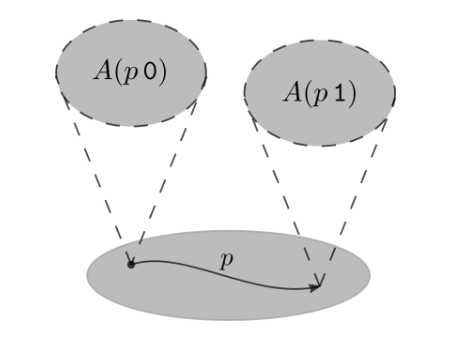
\includegraphics[scale=0.5]{cchm_fib}
  \end{center}
  \begin{center}
    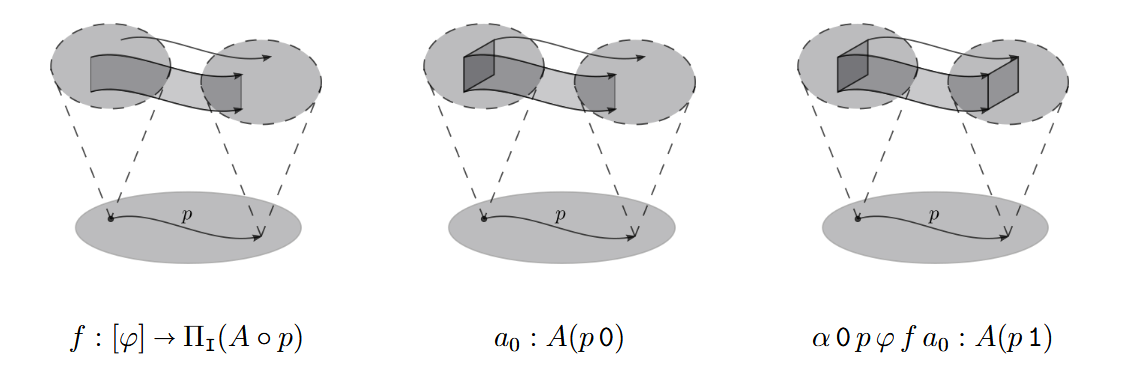
\includegraphics[scale=0.5]{cchm_fib2}
  \end{center}
\end{frame}

\begin{frame}[fragile,shrink]
  令 $\Fib\Gamma$ 为对象$\Gamma$上的 CCHM 纤维化的类型, 定义为
  \[
  \Fib\Gamma\triangleq(A:\Gamma\to\calU)\times\isFib\,A
  \]
  CCHM 纤维化在重索引下是封闭的: 给定$\gamma:\Delta\to\Gamma$ 和 $A:\Gamma\to\calU$, 我们得到一个函数$\_[\gamma]:\isFib\,A\to\isFib(A\circ\gamma)$, 定义为$\alpha[\gamma]\,e\,p\triangleq\alpha\,e\,(\gamma\circ p)$.
\begin{framed}
  $\alpha:\isFib\,A\triangleq(e:\{\ttzero,\ttone\})(p:\ttI\to\Gamma)\to\Comp\,e\,(A\circ p)$
  
  $\alpha[\gamma]:\isFib(A\circ\gamma)\triangleq((e:\{\ttzero,\ttone\})(p:\ttI\to\Delta)\to\Comp\,e\,(A\circ\gamma\circ p)$
\end{framed}
因此我们得到一个函数$\_[\_]:(\Delta\to\Gamma)\to\Fib\Gamma\to\Fib\Delta$, 定义为
\[
(A,\alpha)[\gamma]\triangleq(A\circ\gamma,\alpha[\gamma])
\]
它是函子性的: $(A,\alpha)[id]=(A,\alpha)$ 且 $(A,\alpha)[g\circ f]=(A,\alpha)[g][f]$.
\end{frame}

\begin{frame}[fragile,shrink]{纤维对象}
  我们称$A:\calU$是一个纤维对象, 如果我们有一个关于常数族$\lambda(\ul:1)\to A$ 在终对象 $1$ 上的纤维化结构. 注意: 如果$(A,\alpha):\Fib\Gamma$是一个纤维化, 那么对于每个$x:\Gamma$, 类型$A\,x:\calU$是纤维的, 其纤维化结构由通过映射$\lambda(\ul:1)\to x:1\to\Gamma$对$\alpha$进行重索引得到. 然而, 反过来不成立: 拥有一个纤维化结构的族, 即$(x:\Gamma)\to\isFib(\lambda(\ul:1)\to A\,x)$ 的一个元素, 要弱于拥有一个对于 $A:\Gamma\to\calU$的纤维化结构.
\end{frame}

\begin{frame}[fragile,shrink]{组合结构和填充结构的关系}
  如果$\alpha:\Fill\,e\,A$, 那么$\lambda\varphi\,f\,a\to\alpha\,\varphi\,f\,a\,\overline{e}:\Comp\,e\,A$, 因此每个填充结构都会产生一个组合结构. 反过来, 一个 CCHM 纤维化的组合结构也会产生填充结构: 给定 $\Gamma:\calU$, $A:\Gamma\to\calU$, $e:\{\ttzero,\ttone\}$, $\alpha:\isFib\,A$ 以及 $p:\ttI\to\Gamma$, 存在一个填充结构 $\ttfill\,e\,\alpha\,p:\Fill\,e\,(A\circ p)$, 它在$\overline{e}$处与$\alpha$一致, 即:
  \begin{align*}
    \forall(\varphi:\Cof)(f:[\varphi]\to\Pi_{\ttI}A)&(a:A\,(p\,e)). \\
    &(\varphi,f)\,@\,e\nearrow a \Rightarrow \ttfill\,e\,\alpha\,p\,\varphi\,f\,a\,\overline{e} = \alpha\,e\,p\,\varphi\,f\,a
  \end{align*}
  此外, $\ttfill$ 在重索引下是稳定的, 即对于所有的 $\gamma:\Delta\to\Gamma$ 和 $p:\ttI\to\Delta$
  \[
  \ttfill\,e\,\alpha\,(\gamma\circ p) = \ttfill\,e\,(\varphi[\gamma])\,p
  \]
\end{frame}

\begin{frame}[fragile,shrink]
\begin{verbatim}
----------------------------------------------------------------------
-- Path composition structure
----------------------------------------------------------------------
Comp : OI → (Int → Set) → Set
Comp e A = (φ : Cof)(f : [ φ ] → Π A) →
  ⟦ x₁ ∈ (A ⟨ e ⟩) ∣ (φ , f) ∙ ⟨ e ⟩ ↗ x₁ ⟧ →
  ⟦ x₀ ∈ (A ⟨ ! e ⟩) ∣ (φ , f) ∙ ⟨ ! e ⟩ ↗ x₀ ⟧

----------------------------------------------------------------------
-- Fibrations
----------------------------------------------------------------------
isFib : ∀{a}{Γ : Set a}(A : Γ → Set) → Set a
isFib {Γ = Γ} A = (e : OI)(p : Int → Γ) → Comp e (A ∘ p)

Fib : ∀{a}(Γ : Set a) → Set (lsuc lzero ⊔ a)
Fib {a} Γ = Σ (Γ → Set) isFib

----------------------------------------------------------------------
-- Fibrations can be reindexed
----------------------------------------------------------------------
reindex : ∀{a a'}{Δ : Set a}{Γ : Set a'}(A : Γ → Set)(α : isFib A)(ρ : Δ → Γ) → isFib (A ∘ ρ)
reindex A α ρ e p = α e (ρ ∘ p)

reindex' : ∀{a a'}{Δ : Set a}{Γ : Set a'}(Aα : Fib Γ)(ρ : Δ → Γ) → Fib Δ
reindex' (A , α) ρ = (A ∘ ρ , reindex A α ρ)

----------------------------------------------------------------------
-- Reindexing is functorial
----------------------------------------------------------------------
reindexAlongId : ∀{a}{Γ : Set a}{A : Γ → Set}{α : isFib A} → α ≡ reindex A α id 
reindexAlongId = refl

reindexComp :
  ∀{a b c}{Γ₁ : Set a}{Γ₂ : Set b}{Γ₃ : Set c}{A : Γ₃ → Set}{α : isFib A}
  (f : Γ₁ → Γ₂)(g : Γ₂ → Γ₃)
  → ----------------------
  reindex A α (g ∘ f) ≡ reindex (A ∘ g) (reindex A α g) f
reindexComp g f = refl

reindexAlongId' : ∀{a}{Γ : Set a}{A : Fib Γ} → reindex' A id ≡ A
reindexAlongId' = refl

abstract
 reindexComp' :
  ∀{a b c}{Γ₁ : Set a}{Γ₂ : Set b}{Γ₃ : Set c}
  {A : Fib Γ₃}
  (f : Γ₁ → Γ₂)(g : Γ₂ → Γ₃)
  → ----------------------
  reindex' A (g ∘ f) ≡ reindex' (reindex' A g) f
 reindexComp' g f = refl
\end{verbatim}
\end{frame}

\begin{frame}[fragile,shrink]
\begin{verbatim}
----------------------------------------------------------------------
-- Path filling structure
----------------------------------------------------------------------
Fill : OI → (Int → Set) → Set
Fill e A =
  (φ : Cof)
  (f : [ φ ] → Π A)
  (a : A ⟨ e ⟩)
  (_ : prf ((φ , f) ∙ ⟨ e ⟩ ↗ a))
  → --------------------------------------
  ⟦ p ∈ Π A ∣ ((φ , f ) ↗ p) & (p ⟨ e ⟩ ≈ a) ⟧

----------------------------------------------------------------------
-- Compatible partial functions
----------------------------------------------------------------------
_⌣_ : {A : Set} → □ A → □ A → Ω
(φ , f) ⌣ (ψ , g) = All u ∈ [ φ ] , All v ∈ [ ψ ] , f u ≈ g v

_∪_ :
  {A : Set}
  {φ ψ : Cof}
  (f : [ φ ] → A)
  (g : [ ψ ] → A)
  {p : prf((φ , f) ⌣ (ψ , g))}
  → ---------------------------
  [ φ ∨ ψ ] → A
_∪_ {A} {φ} {ψ} f g {p} w = ∥∥-elim h q w where

  h : [ φ ] ⊎ [ ψ ] → A
  h (inl u) = f u
  h (inr v) = g v

  q : (z z' : [ φ ] ⊎ [ ψ ]) → h z ≡ h z'
  q (inl _) (inl _) = cong f (eq (fst φ))
  q (inl u) (inr v) = p u v
  q (inr v) (inl u) = symm (p u v)
  q (inr _) (inr _) = cong g (eq (fst ψ))
\end{verbatim}
\end{frame}

\begin{frame}[fragile,shrink]{纤维化的性质}
  给定一个类型族$A:\Gamma\to\calU$和一个纤维化$(B,\beta):\Fib\Gamma$, 使得$A\cong B$, 那么我们可以构造 $\alpha$ 使得 $(A,\alpha):\Fib\Gamma$.
\end{frame}
\end{document}